\chapter{نتایج و جمع‌بندی} \label{sec:result}

\section{جمع‌بندی}
در فصول قبل جزئیات و مواردی که برای طراحی و ساخت این ساعت هوشمند مورد نیاز بود شرح داده شد. در نهایت با ترکیب این موارد و انتقال برنامه‌های نوشته شده به ریزپردازنده، پروژه تکمیل شد. تصاویر \ref{fig:reals} ساعت را از نماهای مختلف نشان می‌دهد.

 \begin{figure}[h]
	\centering
	\begin{subfigure}{0.48\textwidth}
		\centering
		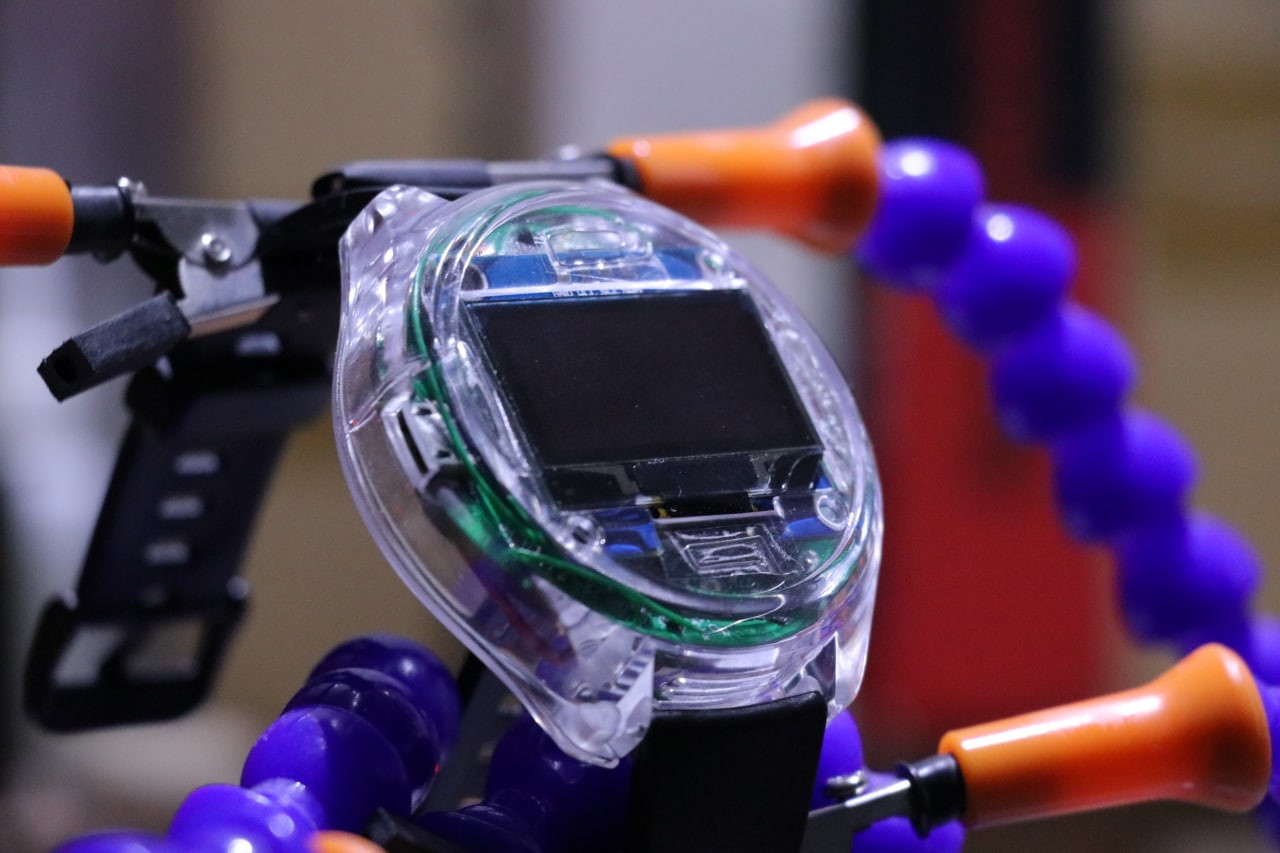
\includegraphics[width=\linewidth]{watch_3d}
		\caption{}
		%\label{fig:stm32_image}
	\end{subfigure}
	\begin{subfigure}{0.48\textwidth}
		\centering
		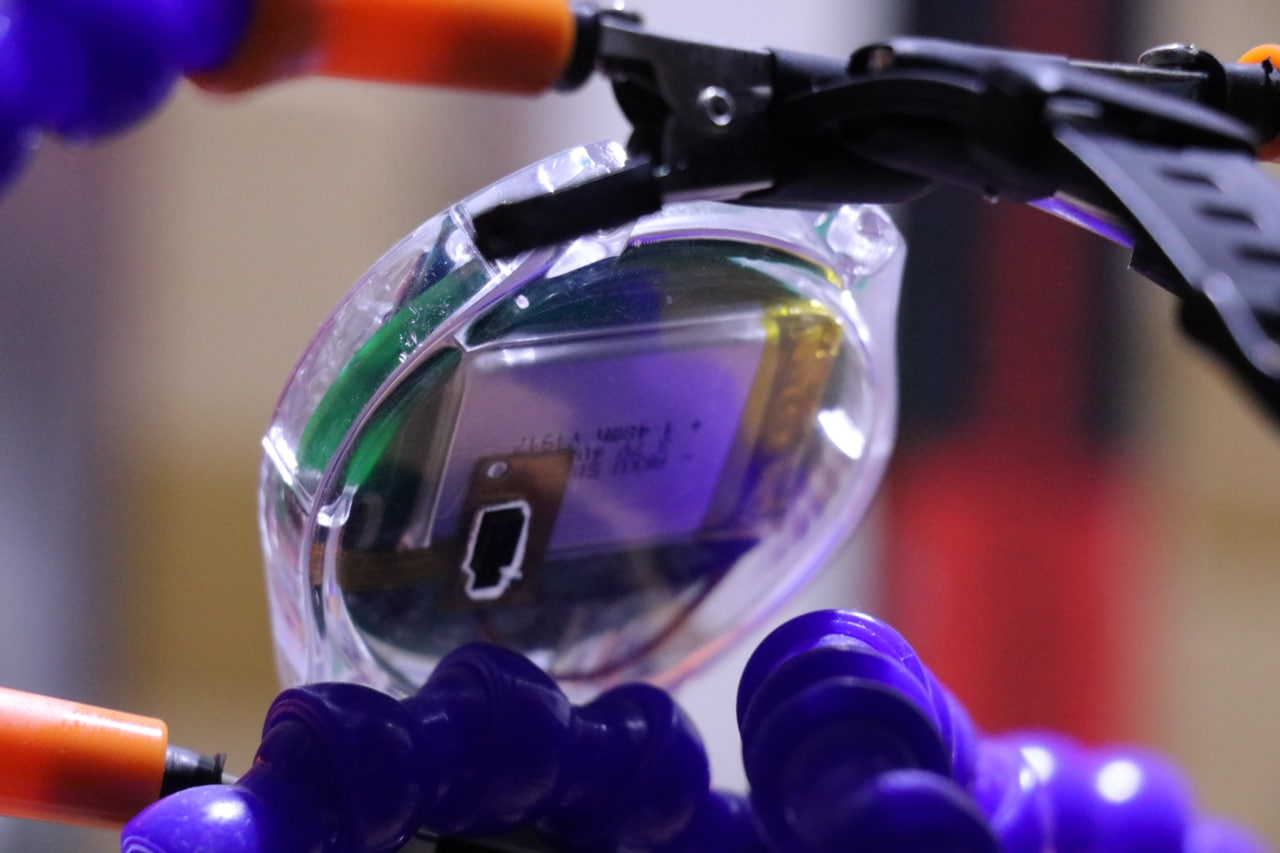
\includegraphics[width=\linewidth]{watch_back}
		\caption{}
		%\label{fig:stm32_real}
	\end{subfigure} \\
	\begin{subfigure}{0.48\textwidth}
		\centering
		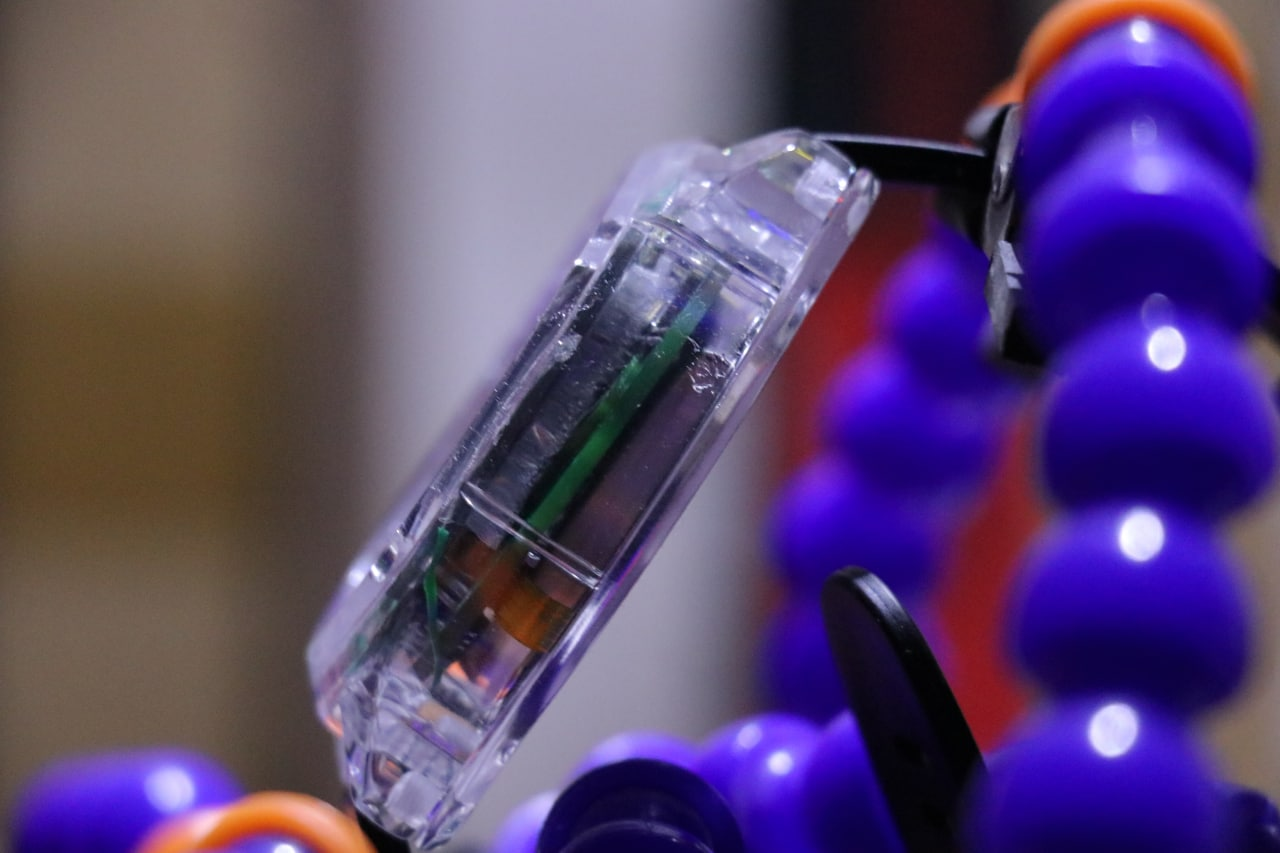
\includegraphics[width=\linewidth]{watch_side2}
		\caption{}
		%\label{fig:stm32_image}
	\end{subfigure}
	\begin{subfigure}{0.48\textwidth}
		\centering
		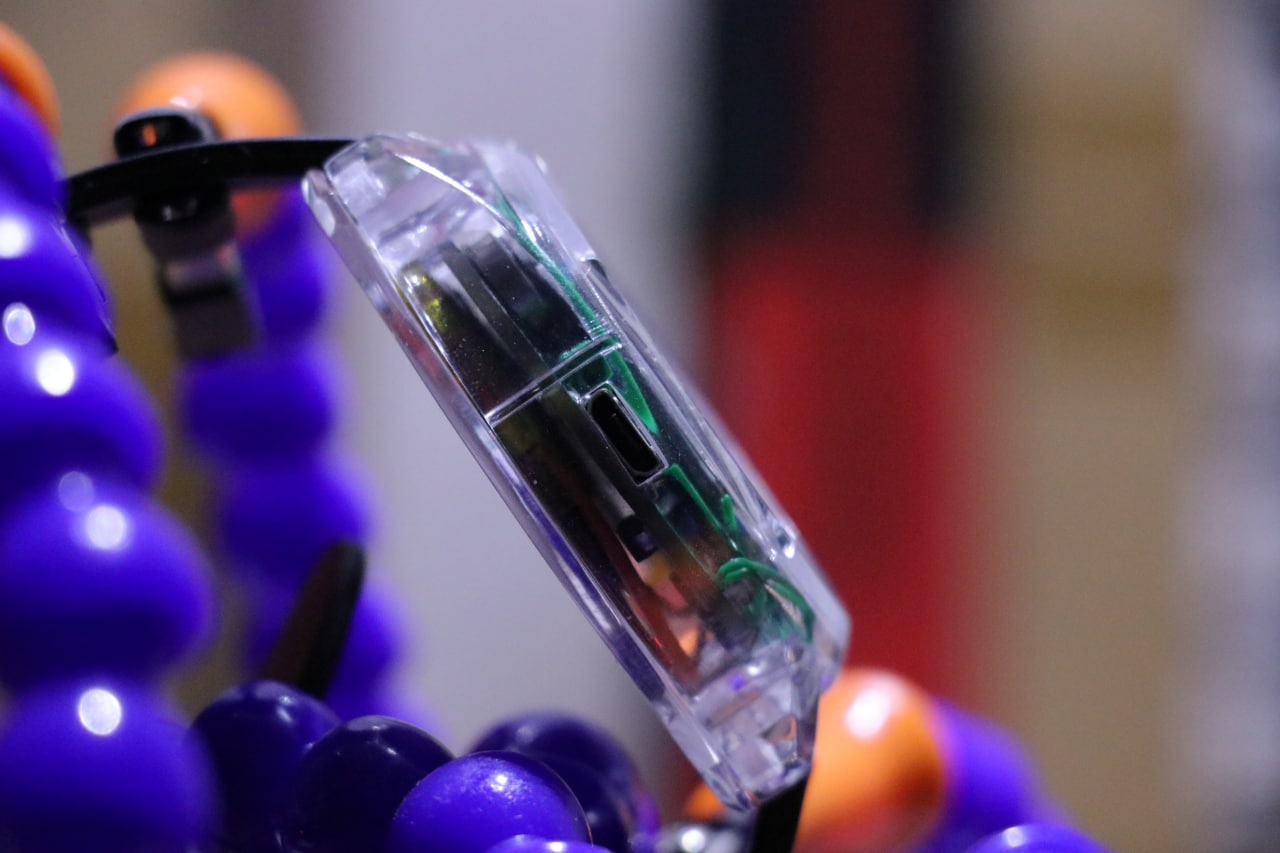
\includegraphics[width=\linewidth]{watch_side1}
		\caption{}
		%\label{fig:stm32_image}
	\end{subfigure}
	\caption{تصاویر محصول نهایی از چند نما}
	\label{fig:reals}
\end{figure}

\section{بهبودها و نقشه‌راه آینده}
در بخش پردازش داده‌های حسگر حرکتی، برای قدم شماری صرفا از شتاب خطی در راستای محور $x$ استفاده شده است. می‌توان برای افزایش دقت و عملکرد، سرعت زاویه‌ای حول محور $z$ را نیز به کار گرفت. به صورتی که به طور مشابه برای این سرعت زاویه‌ای نیز یک شرط هیسترزیسی وضع شود و خروجی آن با خروجی حالت فعلی \lr{AND} شود.

همچنین اگر قدرت پردازشی و حافظه کافی باشد، می‌توان از روش‌های مرسوم تشخیص الگو مانند میان-همبستگی\footnote{\lr{Cross-correlation}}
یا میان-همبستگی بی‌طرفانه\footnote{\lr{Unbiased Cross-correlation}}
بین سیگنال حسگر و سیگنال مرجع نیز بهره برد که عملکرد بهتری ارائه می‌دهند. همچنان روش‌های مبتنی بر یادگیری و شبکه‌های عصبی نیز قابل بررسی هستند.

\section{دسترسی به بخش‌های پروژه}
در نهایت تمام بخش‌های پروژه اعم از فایل‌های طراحی سخت‌افزار، طراحی بدنه و تمام کدهای نوشته شده به صورت متن-باز\footnote{\lr{Open source}}
در سایت \lr{Github} به نشانی
\href{http://smotlaq.ir/IPyEt}{\texttt{https://github.com/SMotlaq/open-watch}}
بارگذاری شده است. توسعه‌دهندگان و علاقمندان به مشارکت و بهبود بخش‌های مختلف پروژه می‌توانند در
\href{http://smotlaq.ir/IPyEt}{صفحه‌ی مربوطه}
درخواست ادغام\footnote{\lr{Merge request / Pull request}}
ارسال نمایند.

\begin{figure}[h]
	\centering
	\href{http://smotlaq.ir/IPyEt}{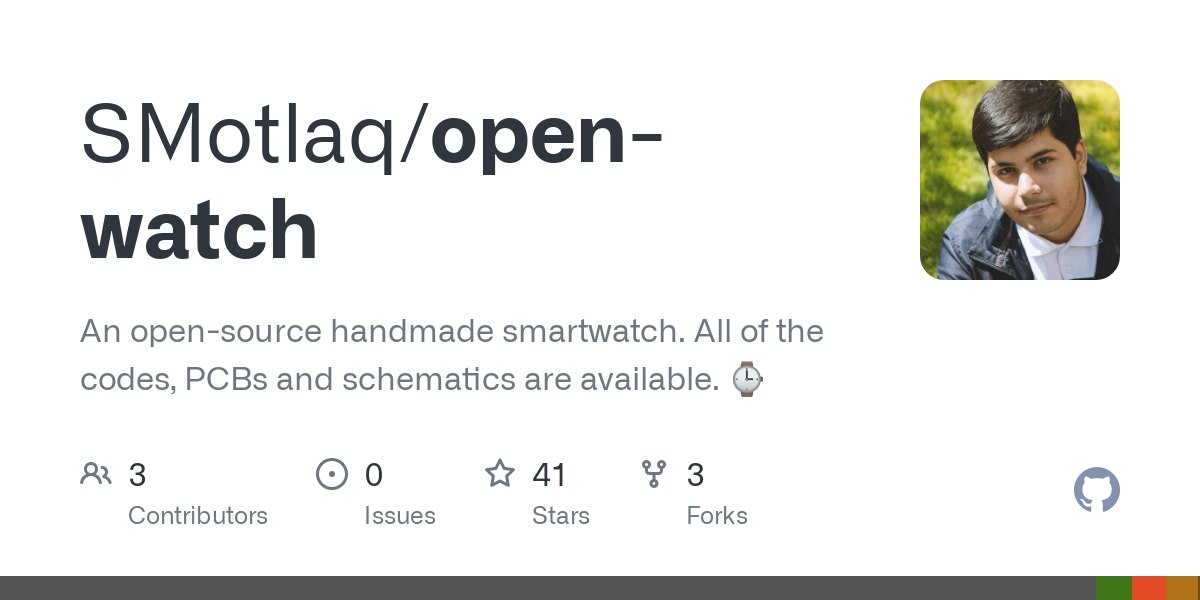
\includegraphics[width=\linewidth]{git}}
	\caption{نشانی پروژه در \lr{Github} و اطلاعات آن}
	\label{fig:git}
\end{figure}
